\documentclass{article}
\usepackage{graphicx} % Required for inserting images
\usepackage{amsmath}
\usepackage{hyperref}

\usepackage{float}
\title{Valutazione sperimentale di diverse oscillazioni accoppiate}
\author{Alessandro Di Meglio \\ Francesco Angelo Fabiano Antonacci}
\date{\today}
\begin{document}

\maketitle

\section{Scopo dell'esperienza} 

Lo scopo dell'esperienza è quello di confrontare e valutare diverse oscillazioni, correlandole fra loro e studiando analogie e differenze.
I tipi di oscillazioni da studiare, con i rispettivi obiettivi da verificare sono:

\begin{itemize}

	    \item OSCILLAZIONE DI UN PENDOLO SINGOLO: confrontare la pulsazione angolare $\omega_{0}$  misurata con la pulsazione angolare teorica.
	    \item OSCILLATORE DI UN PENDOLO SINGOLO SMORZATO: medesimo scopo della misura precedente ma disponendo un galleggiante.
	    \item OSCILLAZIONE IN FASE: misurazione della pulsazione $\omega_{f}$, verificare che $\omega_0 \sim \omega_f$.
	    \item OSCILLAZIONE IN CONTROFASE: misurazione della pulsazione $\omega_{c}$, verificare che $\omega_c \gg \omega_f$.
	    \item BATTIMENTI: misurazione delle pulsazioni angolari portante e modulante da confrontare poi con $\omega_{f}$ e $\omega_{c}$.
    
\end{itemize}

\section{Cenni teorici}

            Adottiamo l'approssimazione delle piccole oscillazioni per semplificare il modello.
            
		\subsection{ Oscillazione di un pendolo singolo}
  
            Le oscillazioni di questa sezione sono date dalla seguente relazione :


\begin{equation}
x(t) = A \cos(w t + \phi) + c
\label{eq:pene_singolo}
\end{equation}  

            La relazione tra pulsazione $w0$,  inerzia $I$,massa $m$, accelerazione di gravità $g$, posizione de centro di massa $x_cm$è la seguente:
            
\begin{equation}
w0 = \sqrt{\frac{m g x_cm}{I}}
\label{eq:w0_teoria}
\end{equation}                    
        
                    
		\subsection{  Oscillatore di un pendolo singolo smorzato }
              Le oscillazioni di questa sezione sono date dalla seguente relazione dove è presente un esponenziale che descrive lo smorzamento dell'oscillazione data dall'attrito viscoso fra galleggiante e acqua
                    
\begin{equation}
x(t) = A e^{-\frac{t}{\tau}} \cos(w  t + \phi) + c                     
\label{eq:pene_smorzato}
\end{equation} 

In questa equazione,  $A$  rappresenta l'ampiezza iniziale, $\omega$  è la pulsazione , $\phi$  è la fase dell'oscillazione, $c$  è la costante di spostamento, e $\tau$  è il tempo caratteristico del decadimento esponenziale.
                    
		\subsection{  Oscillazioni in fase}
                La relazione tra posizione e tempo di ciascuno dei due pendoli in fase è come sopra (\ref{eq:pene_smorzato} ). E' stato deciso di adottare il modello del pendolo smorzato per quanto detto nella sezione (\ref{sez:modello}).
                
                Si può dimostrare che :$\omega_0 \sim \omega_f$
                                
		\subsection{  Oscillazioni in controfase}
                 La relazione tra posizione e tempo di ciascuno dei due pendoli in controfase è come sopra (\ref{eq:pene_smorzato} ).	 E' stato deciso di adottare il modello del pendolo smorzato per quanto detto nella sezione (\ref{sez:modello}).

                 Si può dimostrare che :$\omega_c > \omega_f$
                 
            \subsection{  Battimenti}
                 La relazione tra posizione e tempo di ciascuno dei due pendoli nel caso in cui si osservino i battimenti è:
                 
 \begin{equation}
x(t) = 2A_0 \cos(\omega_p t + \phi_p) \cos(\omega_b t + \phi_b) + c
\label{eq:bat}
\end{equation}

In questa equazione,  $A_0$  rappresenta l'ampiezza iniziale, $\omega_p$  è la pulsazione più rapida,$ \omega_b$  è la pulsazione più lenta, $\phi_p$  è la fase dell'oscillazione più rapida, $\phi_b$  è la fase dell'oscillazione più lenta, $c$  è la costante di spostamento, e $\tau$  è il tempo caratteristico del decadimento esponenziale.

Ci si aspetta dalla teoria le seguenti relazioni:

\begin{equation}
    \omega_p=\frac{\omega_f+\omega_c}{2}
    \label{eq:wp}
\end{equation}

\begin{equation}
    \omega_b=\frac{\omega_f-\omega_c}{2}
    \label{eq:wb}
\end{equation}

Dove $\omega_f$ è la frequenza dei due pendoli in  fase, $\omega_c$ è la frequenza dei due pendoli in  controfase.


\section{Apparato strumentale}

			\begin{itemize}
                          \item due pendoli 
                          \item supporto con vasca di acqua sottostante
					   \item galleggiante da pesca 
					   \item molla 
					   \item Metro a nastro con risoluzione di 1 mm 
					   \item calibro Palmer con risoluzione di 0.05 mm
					   \item sistema di presa dati con Arduino
			\end{itemize}

\section{Descrizione delle misure}
	       
		\subsection{ Misure dimensioni pendoli }
            Un punto preliminare per l'intera esperienza è la misurazione delle dimensioni spaziali dei pendoli, nello specifico la lunghezza dell'asta e i raggi dei cilindri posti alla fine delle sbarre.
            I due pendoli avevano medesime dimensioni, le misure effettuate sono state riportate in tabella(\ref{tab:dimensioni})

            

                \begin{table}[h!]
                    \centering
                            
                            \begin{tabular}{|c|c|}
                            \hline
                               $diametro$[mm]  & $sezione$[mm] \\
                            \hline

                               $69 \pm 1$ &  $12.40\pm0.05$\\
                            \hline
                            \hline

                               $lunghezza$[mm]  & $base$[mm] \\
                            \hline

                                $476\pm5$ & $8.40\pm0.05$ \\
                            \hline
                            \end{tabular}
                    \caption{$diametro$ è il diametro di del cilindro di ottone, $sezione$ spessore del cilindro di ottone. $lunghezza$ è la lunghezza della sbarra del pendolo, $base$ è il lato della sezione quadrata della sbarra.}
                    \label{tab:dimensioni}
                \end{table}

            
		\subsection{ Oscillazione di un pendolo singolo}
            E' stato spostato un solo pendolo dalla sua posizione di equilibrio ed è stato fatto oscillare prendendo i dati con Arduino.
		\subsection{  Oscillatore di un pendolo singolo smorzato }
            È stato posto, a contatto con l'acqua, un galleggiante fissato nella estremità inferiore di un pendolo e il suo scopo è stato quello di smorzare le oscillazioni. 
            E' stato spostato il pendolo dalla sua posizione di equilibrio ed è stato fatto oscillare prendendo i dati con Arduino.
            
		\subsection{  Oscillazioni in fase}
  
            Sono stati collegati con una molla due pendoli.
            Sono stati spostati dalla loro posizione di equilibrio della stessa distanza nella stessa direzione, sono stati lasciati oscillare, sono state prese le posizioni dei due con Arduino.
            
		\subsection{  Oscillazioni in controfase}
  
            Sono stati collegati con una molla due pendoli e successivamente 
            spostati dalla loro posizione di equilibrio della stessa distanza in direzione opposta, sono stati lasciati oscillare, sono state prese le posizioni dei due con Arduino.
  
		\subsection{  Battimenti}
  
            Sono stati collegati con una molla due pendoli,uno si è 
            spostato dalla posizione di equilibrio, mentre l'altro è stato lasciato fermo. Sono stati lasciati oscillare, sono state prese le posizioni dei due con Arduino.


            
\section{Stima delle incertezze}


  
		\subsection{Incertezze sulle dimensione}

                L'incertezza sulle dimensioni del pendolo riportate in tabella (\ref{tab:dimensioni}) sono la risoluzione del metro a nastro e del calibro ventesimale con cui sono state prese le misure.

                
		\subsection{Incertezze sulle posizioni}
  
                Le incertezze sulle posizioni $s$ sono date dalla deviazione standard della distribuzione lineare di ampiezza la risoluzione di Arduino, $\sigma_s=0.3$ [u.a.] (unità arbitraria), trascurabile al fine del nostro esperimento.
		
            \subsection{Incertezze sui tempi}
  
                Medesimo discorso della sottosezione precedente, dunque assumeremo che l'incertezza sui tempi sia di $\sigma_t=0.004$ [s].

    
\section{Analisi dei dati}

            \subsection{ Approssimazioni}
                E' verificata, per due ordini di grandezza, l'ipotesi di piccole oscillazioni utilizzata in (\textbf{Cenni Teorici}):

\begin{equation}
\theta \ll \frac{16\sigma_t}{t}
\label{verifica}
\end{equation}
Dove $\theta$ è l'angolo massimo, $ t$ è il periodo e $\sigma_t$ è l'incertezza sul periodo.
\subsection{Algoritmo di best fit}
    
    E' stato fatto un fit ai minimi quadrati per ciascuna delle leggi.
    Si osserva che l'errore sui tempi $\sigma_t$ non è trascurabile nel best-fit rispetto all'errore sulle posizioni $\sigma_s$:
    
    $$ \sigma_s\ll \frac{df}{dt}\sigma_t $$
    
    Per trascurare l'errore sui tempi è stata utilizzata un'incertezza efficace sulle posizioni ottenuta sommando in quadratura quella delle posizioni con quello sui tempi moltiplicato per una stima della velocità istantanea in ciascun punto.
    A posteriori, per la presenza di errori sistematici, si osserva che le ipotesi del fit ai minimi quadrati non sono state verificate per tutti i modelli eccetto: il pendolo smorzato nella configurazione del pendolo semplice e il modello e la configurazione dei battimenti.



                

            \subsection{ Oscillazione di un pendolo singolo}
              In tabella (\ref{tab:pendolosingolo}) sono riportati i parametri trovati dall'algoritmo di best-fit.
              In figura(\ref{fig:ps}) e in figura (\ref{fig:psres}) sono riportate rispettivamente  le misure con il best-fit e il grafico dei residui.



                \begin{table}[h! ]
                        \centering
                        \caption{Dati del Pendolo Singolo}
                        \begin{tabular}{|l|c|}
                        \hline
                        Parametro & Valore \\
                        \hline
                        $A$ [u.a.]& $118.24 \pm 0.06$ \\
                        $\omega$[$s^{-1}$] & $4.4318 \pm 0.0004$ \\
                        $\phi$ & $0.693 \pm 0.003$ \\
                        $c$[u.a.]  & $529.88 \pm 0.06$ \\
                        \hline
                        \end{tabular}
                        \label{tab:pendolosingolo}
                \end{table}

                 \begin{figure}[h! ]
                    \centering
                    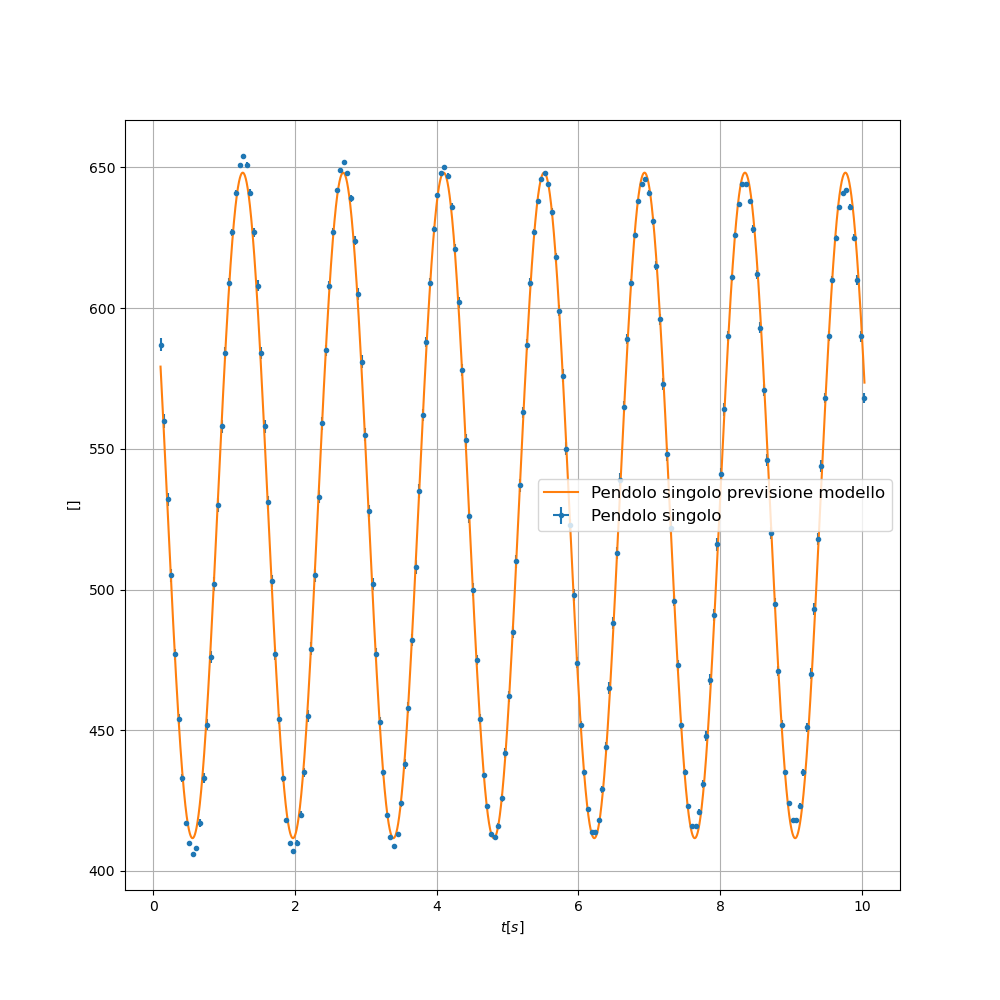
\includegraphics[width=1\linewidth]{Pendolo singolo.png}
                    \caption{Pendolo singolo}
                    \label{fig:ps}
                \end{figure}
    
                \begin{figure}[h! ]
                    \centering
                    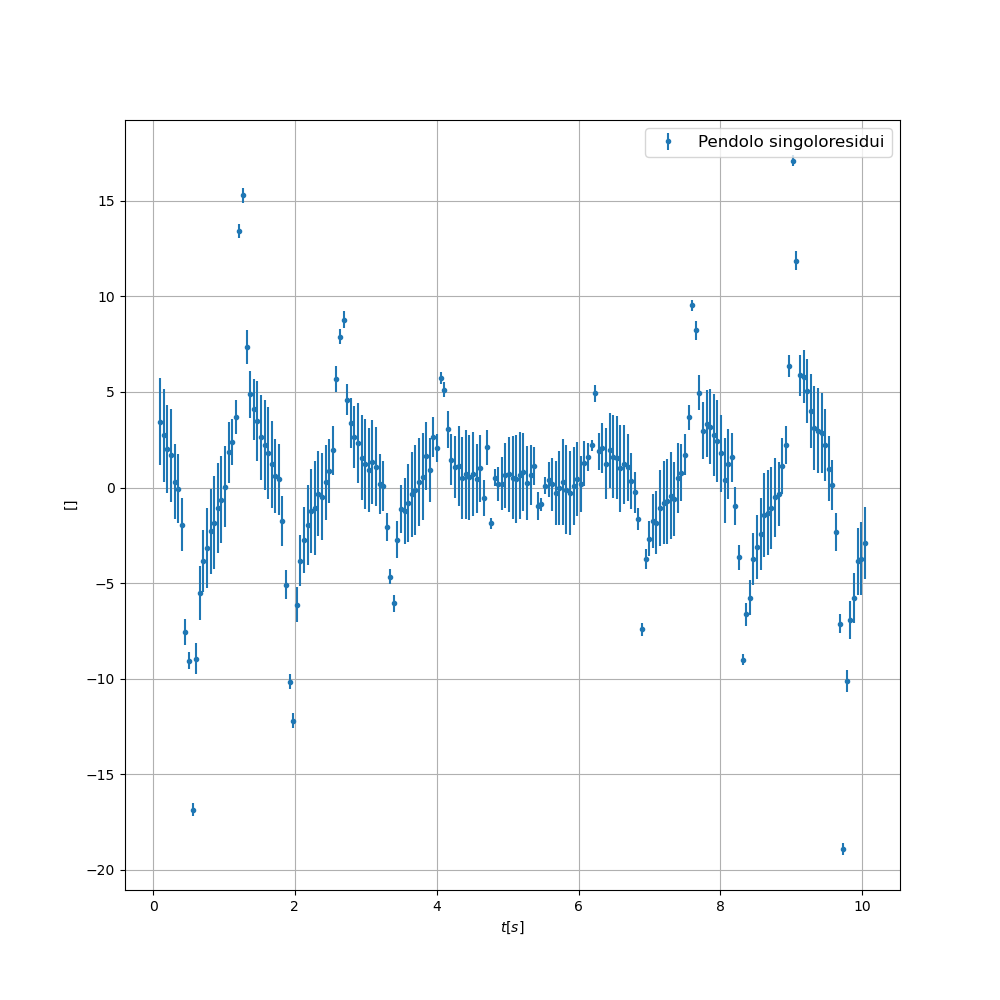
\includegraphics[width=1\linewidth]{Pendolo singolo_residuals.png}
                    \caption{Pendolo singolo residui}
                    \label{fig:psres}
                \end{figure}

            I dati ottenuti dall'esperienza sono in accordo, distando di  una barra di errore e mezzo, con il modello teorico dell'equazione (\ref{eq:w0_teoria}):  $\omega0=4.46 \pm 0.02 s^{-1}$.

            \subsubsection{Valutazione del modello}
            
             Oltre che dal $\chi^2$ , dal grafico dei residui si osserva che il modello è inadeguato a modellizzare le oscillazioni: le permanenze e le variazioni, oltre che all'evidente oscillazione dei dati mostrano che gli le oscillazioni attorno al valore previsto dal modello sono tra loro correlate.
             Segue che è privo di significato riportare $\chi^2$ e $p-value$.


\subsection{ Oscillazione di un pendolo singolo col modello del pendolo smorzato}
              In tabella (\ref{tab:pendolosingolobetter}) sono riportati i parametri trovati dall'algoritmo di best-fit.
              In figura(\ref{fig:ps}) e in figura (\ref{fig:psresbetter}) sono riportate rispettivamente  le misure con il best-fit e il grafico dei residui.



                \begin{table}[h! ]
                        \centering
                        \caption{Dati del Pendolo Singolo}
                        \begin{tabular}{|l|c|}
                        \hline
                        Parametro & Valore \\
                        \hline
                        $A$ [u.a.]& $125.7 \pm 0.1$ \\
                        $\omega$[$s^{-1}$] & $4.4400 \pm 0.0003$ \\
                        $\phi$ & $0.654 \pm 0.002$ \\
                        $c$[u.a.]  & $530.31 \pm0.05$ \\
                        $\tau$[s]  & $85 \pm 2$ \\
                        \hline
                        \end{tabular}
                        
                        \label{tab:pendolosingolobetter}

                \end{table}

                 \begin{figure}[h! ]
                    \centering
                    \includegraphics[width=1\linewidth]{Pendolo_singolo_smorzato_better.png}
                    \caption{Pendolo singolo con modello del pendolo smorzato}
                    \label{fig:psbetter}
                \end{figure}
    
                \begin{figure}[h! ]
                    \centering
                    \includegraphics[width=1\linewidth]{Pendolo_singolo_smorzato_better.png}
                    \caption{Pendolo singolo con modello del pendolo smorzato residui }
                    \label{fig:psresbetter}
                \end{figure}

            I dati ottenuti dall'esperienza sono in accordo, distando di  una barra di errore, meno del modello precedente, con il modello teorico dell'equazione (\ref{eq:w0_teoria}):  $\omega0=4.46 \pm 0.02 s^{-1}$.
        

            \subsubsection{Valutazione del modello}
            
             Dal grafico dei residui non vi è motivo di sospettare la bontà del modello né la presenza di errori sistematici.
             Si riportano il $\chi^2$ e il $p_{value}$ : $\chi^2= 160 p_{value}= 0.05 Dof= 192 $
             

           



		\subsection{  Oscillazione di un pendolo singolo smorzato }
    In tabella (\ref{tab:pm}) riportiamo i parametri trovati dall'algoritmo di best-fit.
              In figura(\ref{fig:pm}) e in figura (\ref{fig:pmres}) sono riportate rispettivamente  le misure con il best-fit e il grafico dei residui. 
               

                \begin{table}[h! ]
                        \centering
                        \caption{Dati del Pendolo Singolo Smorzato}
                        \begin{tabular}{|c|c|}
                        \hline
                        Parametro & Valore \\
                        \hline
                        $A $ [u.a.] & $124.0 \pm 0.1$ \\
                        $\omega$ [$s^{-1}$]& $4.4238 \pm 0.0005$ \\
                        $\phi$& $-1.316 \pm 0.003$ \\
                        $c$[u.a.] & $440.98 \pm 0.06$ \\
                        $\tau$ [s]& $28.2 \pm 0.2$\\
                        \hline
                        \end{tabular}
                        
                        \label{tab:pm}
                       
                \end{table}



            \begin{figure}[h! ]
                \centering
                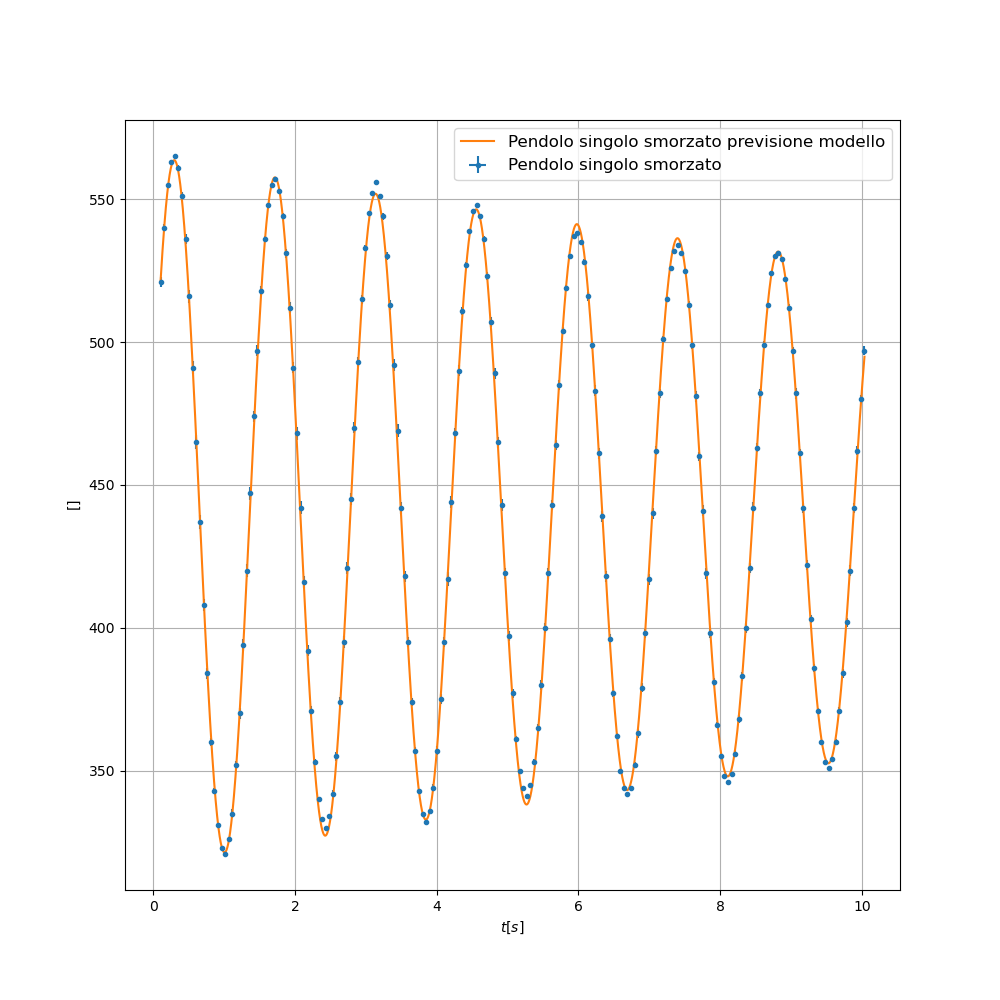
\includegraphics[width=1\linewidth]{Pendolo singolo smorzato.png}
                \caption{Pendolo singolo smorzato}
                \label{fig:pm}
            \end{figure}
            
            \begin{figure}[h! ]
                \centering
                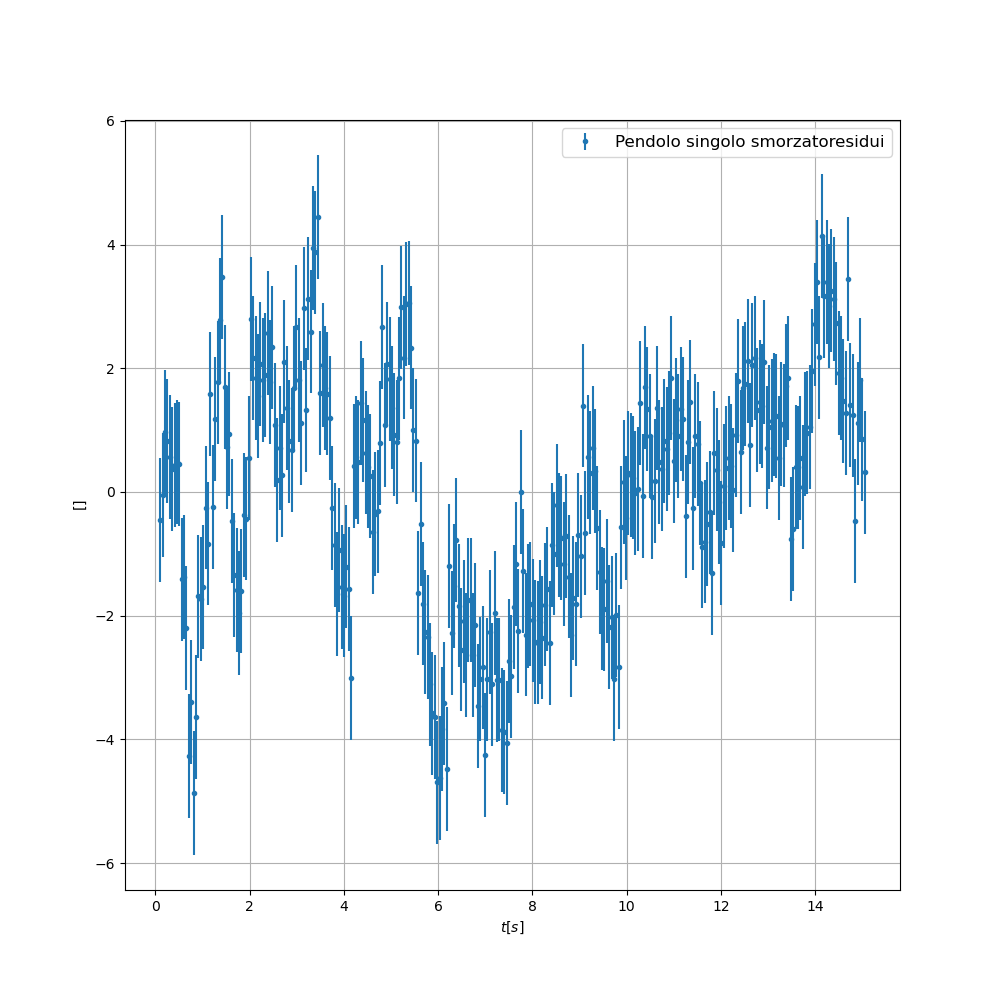
\includegraphics[width=1\linewidth]{Pendolo singolo smorzato_residuals.png}
                \caption{Pendolo singolo smorzato residui}
                \label{fig:pmres}
            \end{figure}


            Si osserva che la misura della pulsazione del pendolo smorzato, si trova a circa venti barre di errore dalla pulsazione del pendolo semplice: supposto che le misure siano state prese facendo partire i pendoli dalla stessa ampiezza, è ragionevole affermare che il periodo sia diminuito a causa dello smorzamento.
            E' ragionevole supporre che sia necessario modificare il modello per tenere conto della variazione del periodo dovuto allo smorzamento.
        



            \subsubsection{Valutazione del modello}
            \label{sez:modello}
            Dal $\chi^2$ , dal grafico dei residui si osserva che il modello è inadeguato a modellizzare le oscillazioni: le permanenze e le variazioni, oltre che all'evidente oscillazione dei dati mostrano che le oscillazioni attorno al valore previsto dal modello sono tra loro correlate.
             Segue che è privo di significato riportare $\chi^2$ e $p-value$.
             
             
             









            
		\subsection{  Oscillazioni in fase}

    
  In tabella (\ref{tab:pf}) riportiamo i parametri trovati dall'algoritmo di best-fit.
              In figura(\ref{fig:pf}) e in figura (\ref{fig:pfres}) sono riportate rispettivamente  le misure con il best-fit e il grafico dei residui. 
    
                \begin{table}[h! ]
                        \centering
                        \caption{Pendolo in Fase}
                        \begin{tabular}{|l|c|}
                        \hline
                        Parametro & Valore \\
                        \hline
                        $A$[u.a.] & $127.5 \pm 0.1$ \\
                        $\omega$[$s^{-1}$] & $4.4392 \pm 0.0005$ \\
                        $\phi$ & $-0.482 \pm 0.003$ \\
                        $c$ [u.a.]& $485.83 \pm 0.05$ \\
                        $\tau$ [s] & $66.5 \pm 0.8$ \\
                        \hline
                        \end{tabular}
                        \label{tab:pf}
                        
                \end{table}


            \begin{figure}[h! ]
                \centering
                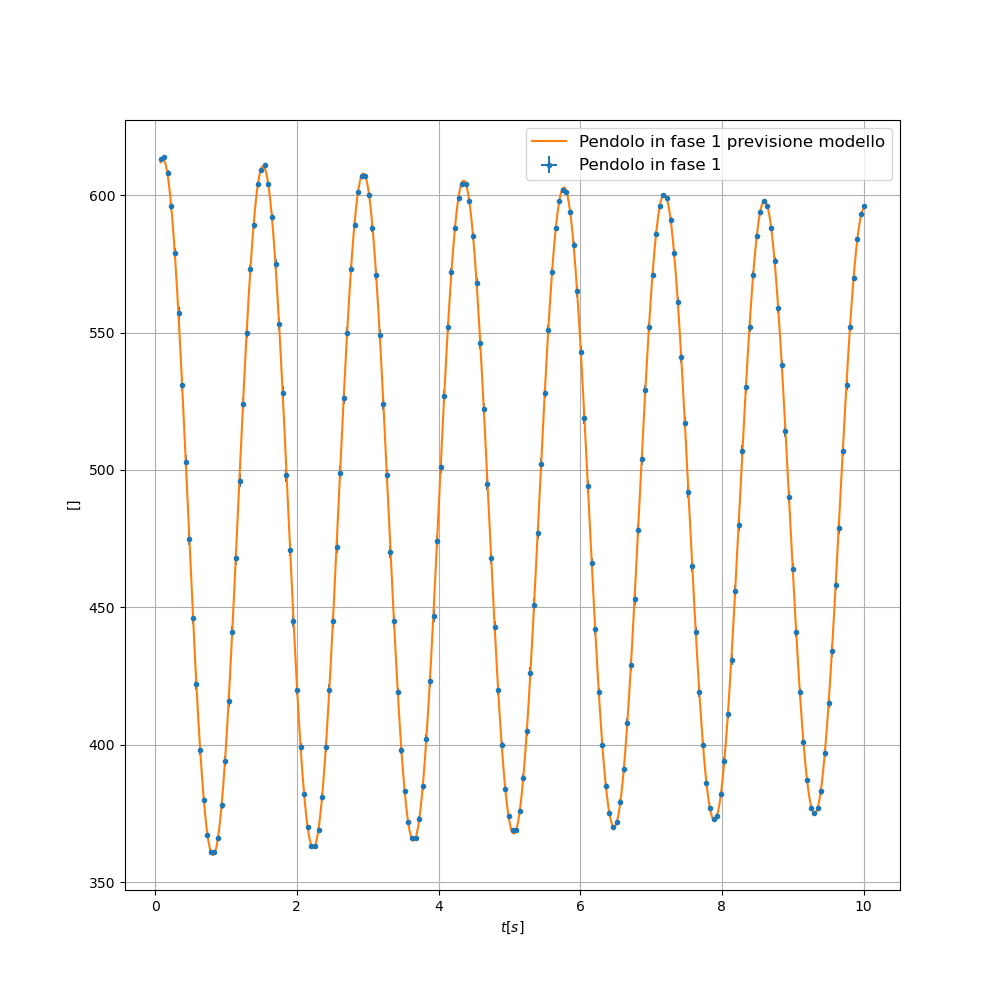
\includegraphics[width=1\linewidth]{Pendolo in fase 1.png}
                \caption{Pendolo in fase 1}
                \label{fig:pf}
            \end{figure}
            
            \begin{figure}[h! ]
                \centering
                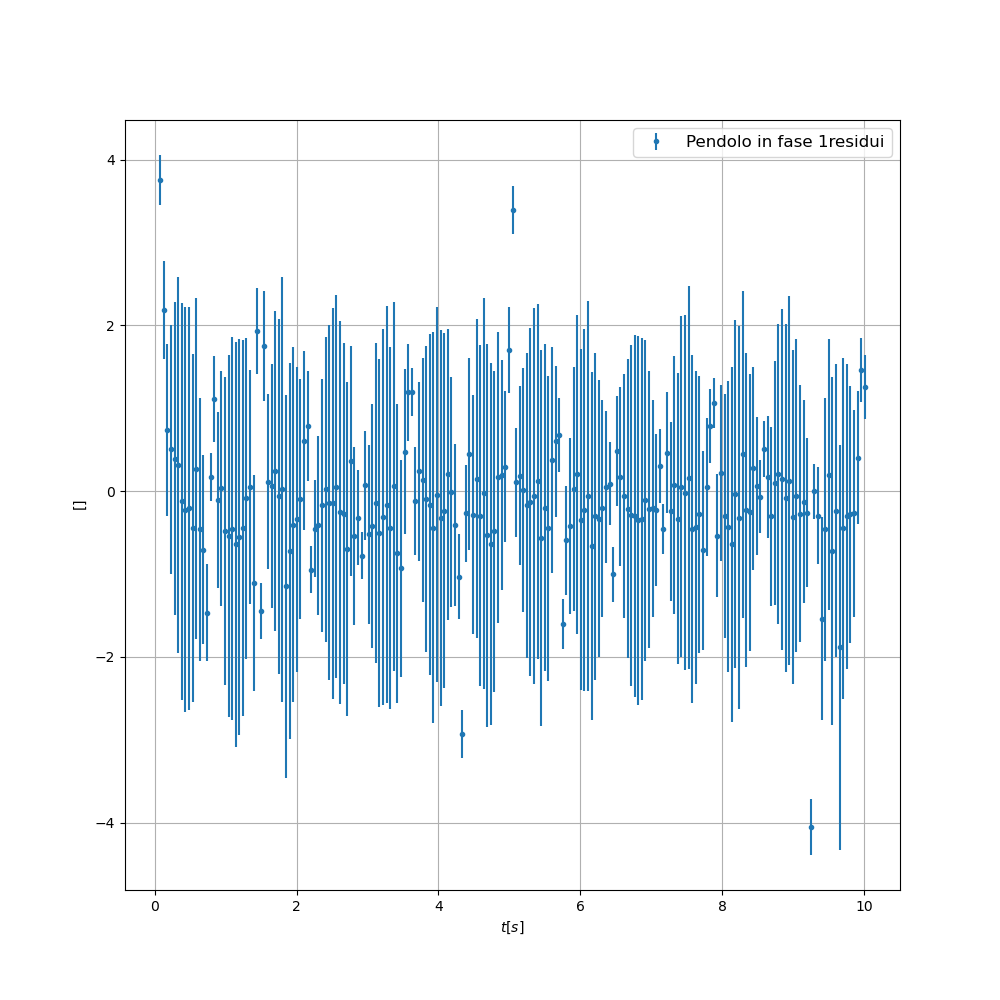
\includegraphics[width=1\linewidth]{Pendolo in fase 1_residuals.png}
                \caption{Pendolo in fase 1 residui}
                \label{fig:pfres}
            \end{figure}


            Si osserva che la misura della pulsazione dei pendoli in fase, si trova a circa una barra di errore dalla misura sulla pulsazione dell'oscillatore singolo.
        

            \subsubsection{Valutazione del modello}
          
             Dal grafico dei residui si osserva che il modello è inadeguato a modellizzare le oscillazioni: le permanenze e le variazioni, oltre che all'evidente oscillazione dei dati mostrano che le oscillazioni attorno al valore previsto dal modello sono tra loro correlate.
             Si osserva che il termine che è stato aggiunto per considerare l'attrito, nonostante non abbia risolto il problema delle oscillazioni delle misure attorno al valore atteso dal modello, ha sensibilmente ridotto la distanza tra dati e modello.
             Si osserva, in un campionamento più ampio di quello  riportato in figura \ref{fig:pf}, anche un lieve fenomeno di battimenti.
             Segue che è privo di significato riportare $\chi^2$ e $p-value$.

           

    
		\subsection{  Oscillazioni in contro-fase}
    In tabella (\ref{tab:pc}) riportiamo i parametri trovati dall'algoritmo di best-fit.
              In figura(\ref{fig:pc}) e in figura (\ref{fig:pcres}) sono riportate rispettivamente  le misure con il best-fit e il grafico dei residui. 

                \begin{table}[h!]
                    \centering
                    \caption{Pendolo in Contro-fase}
                    \begin{tabular}{|l|c|}
                            \hline
                            Parametro & Valore \\
                            \hline
                            $A$ [u.a.]& $140.1 \pm 0.1$ \\
                            $\omega$[$s^{-1}$] & $4.6018\pm 0.0005$ \\
                            $\phi$ & $-1.370 \pm 0.003$ \\
                            $c$ [u.a.] & $489.82 \pm 0.06$ \\
                            $\tau$ [s] & $42.5 \pm 0.3$ \\
                            \hline
                            
                    \end{tabular}
                    \label{tab:pc}
                \end{table}


                \begin{figure}[h!]
                    \centering
                    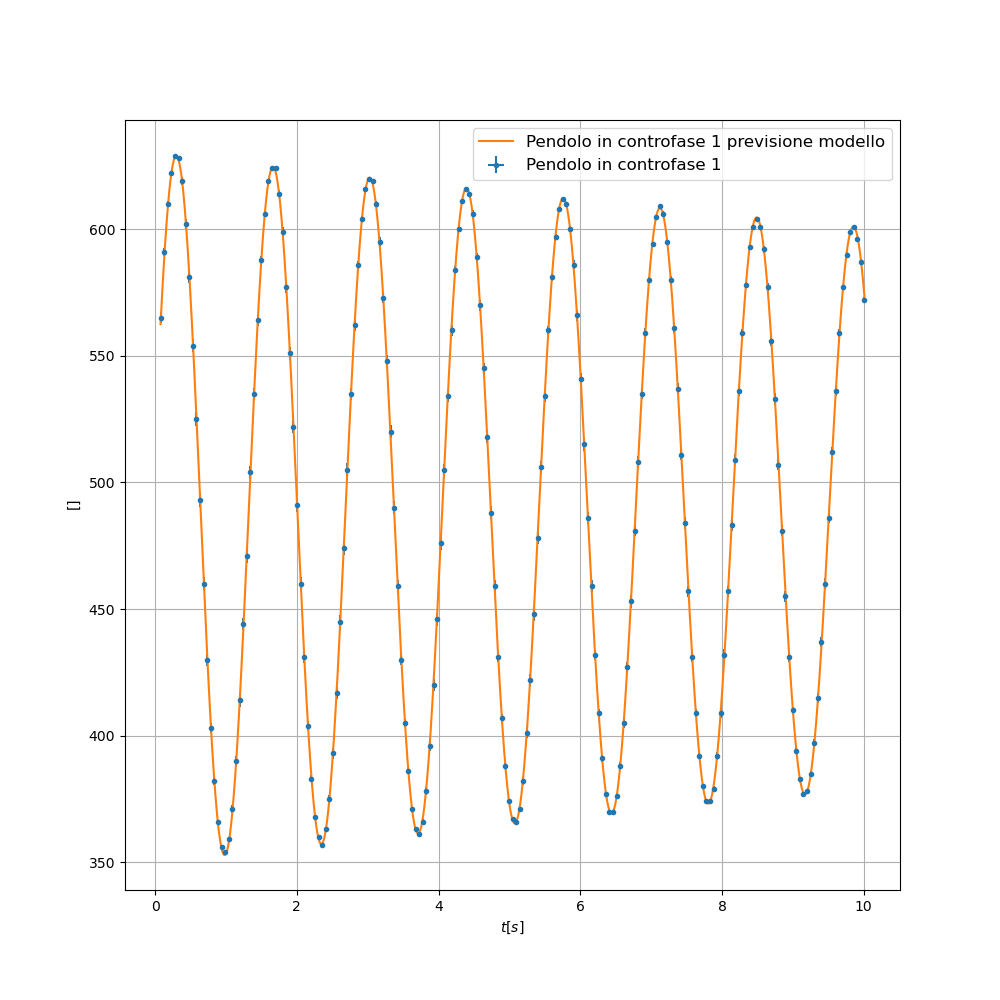
\includegraphics[width=1\linewidth]{Pendolo in controfase 1.png}
                    \caption{Pendolo in contro-fase 1}
                    \label{fig:pc}
                \end{figure}

                \begin{figure}[h! ]
                    \centering
                    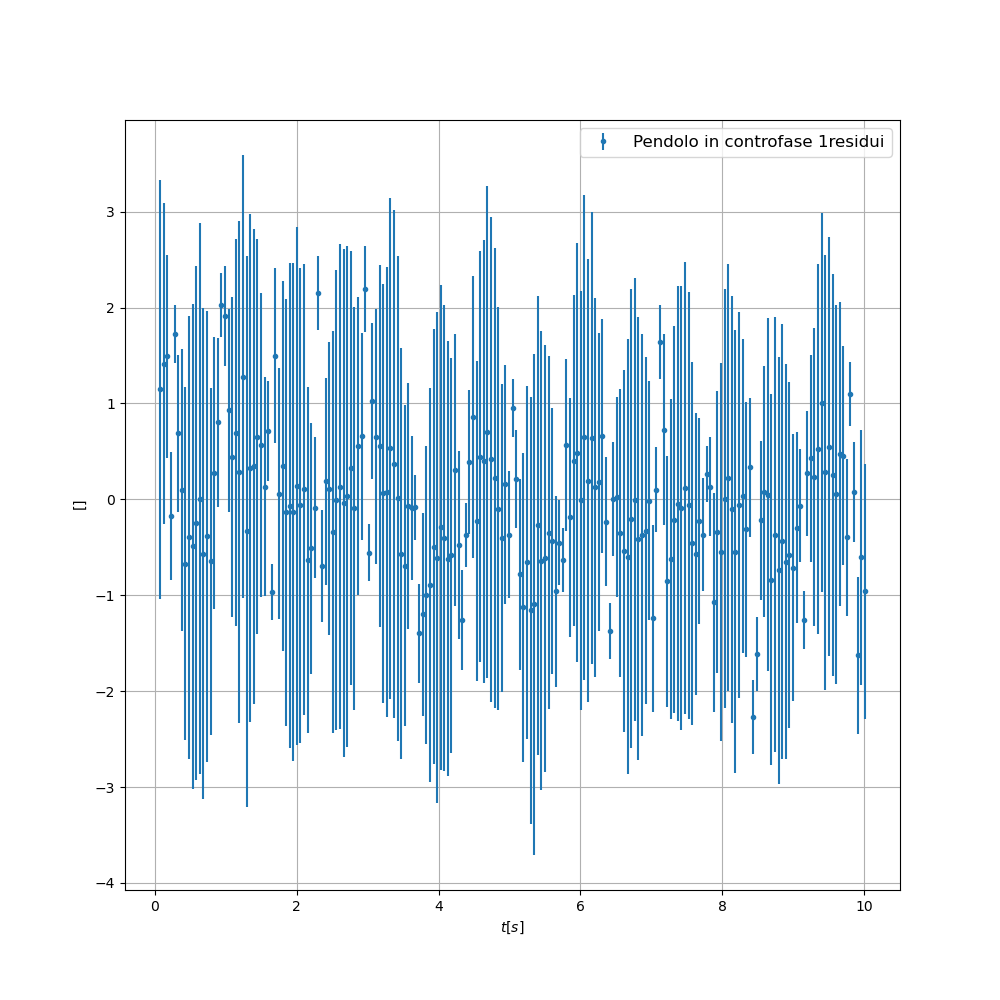
\includegraphics[width=1\linewidth]{Pendolo in controfase 1_residuals.png}
                    \caption{Pendolo in contro-fase residui 1}
                    \label{fig:pcres}
                \end{figure}

            Si osserva che la misura della pulsazione dei pendoli in contro-fase è incompatibile con quella dei pendoli in fase: si trova a circa tre barre di errore sopra.
            E' stato dunque sperimentalmente verificato che $\omega_c \gg \omega_f$.
            
            \subsubsection{Valutazione del modello}
            
              Dal grafico dei residui si osserva che il modello è inadeguato a modellizzare le oscillazioni: le permanenze e le variazioni, oltre che all'evidente oscillazione dei dati mostrano che le oscillazioni attorno al valore previsto dal modello sono tra loro correlate.
             Si osserva, in un campionamento più ampio di quello  riportato in  figura \ref{fig:pc}, anche un lieve fenomeno di battimenti.
             Segue che è privo di significato riportare $\chi^2$ e $p-value$.
           
    
		\subsection{  Battimenti}
  
                In tabella (\ref{tab:pb}) riportiamo i parametri trovati dall'algoritmo di best-fit.
              In figura(\ref{fig:pb}) e in figura (\ref{fig:pbres}) sono riportate rispettivamente  le misure con il best-fit e il grafico dei residui. 
                \begin{table}[h! ]
                    \centering
                    \caption{Battimenti Pendolo 1}
                    \begin{tabular}{|l|c|}
                    \hline
                    Parametro & Valore \\
                    \hline
                    $A$[u.a.] & $ 70 \pm 1$ \\
                    $\omega_p$ [$s^{-1}$]& $4.5861 \pm 0.0007$ \\
                    $\omega_b$ [$s^{-1}$] & $0.074 \pm 0.002$ \\
                    $\phi_p$ & $-0.642 \pm 0.005$ \\
                    $\phi_b$ & $1.731 \pm 0.002$ \\
                    $c$ [u.a.] & $506.90 \pm 0.05$ \\
                    \hline
                    
                    \end{tabular}
                    \label{tab:pb}
                \end{table}


                    \begin{figure}
                        \centering
                        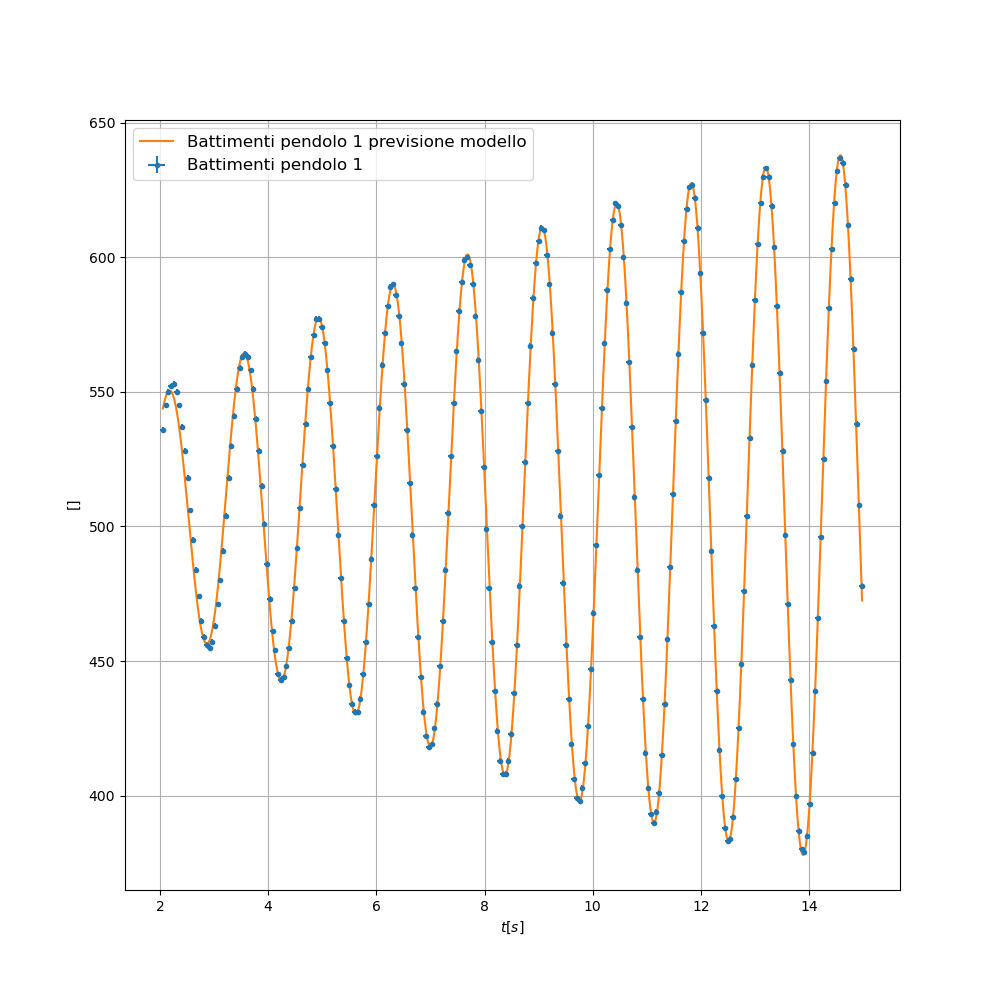
\includegraphics[width=1\linewidth]{Battimenti pendolo 1.png}
                        \caption{Battimenti pendolo 1}
                        \label{fig:pb}
                    \end{figure}
        
        
                    \begin{figure}
                        \centering
                        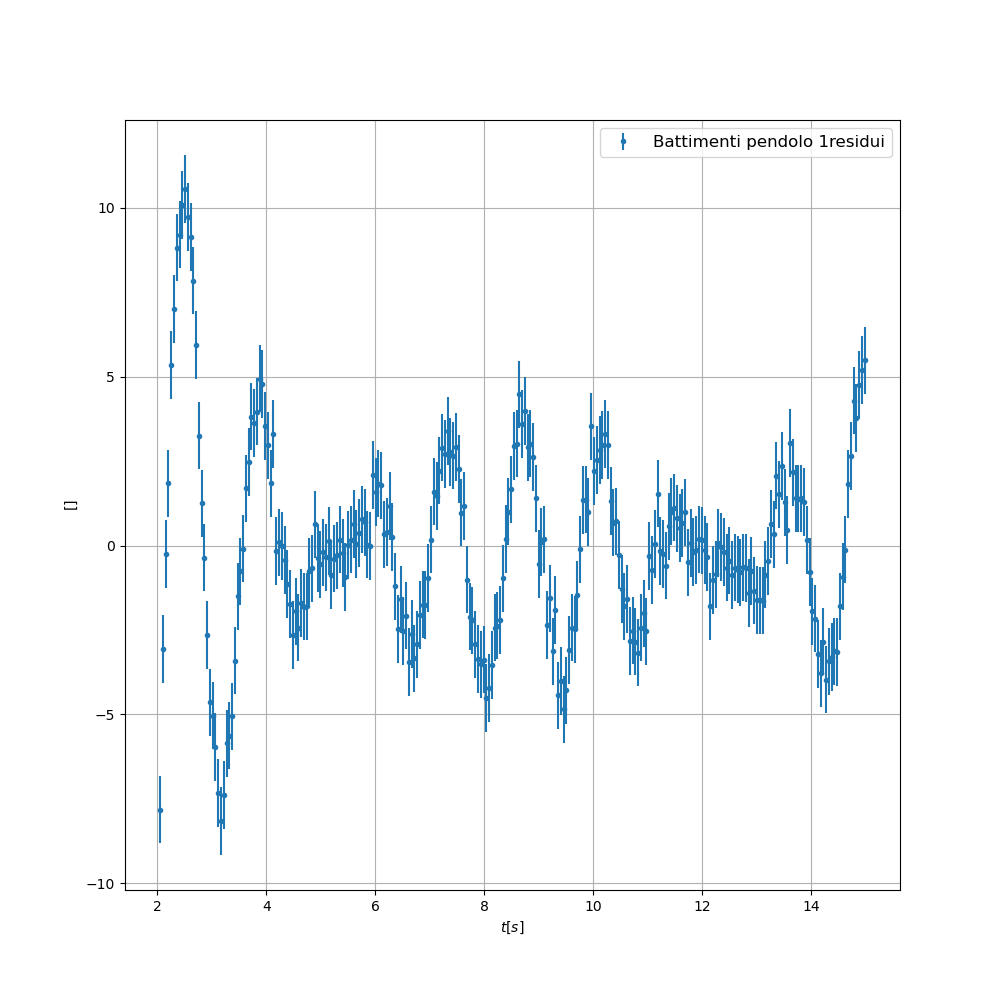
\includegraphics[width=1\linewidth]{Battimenti pendolo 1_residuals.png}
                        \caption{Battimenti pendolo 1 residui}
                        \label{fig:pbres}
                    \end{figure}


                \begin{table}[h! ]
                    \centering
                    \caption{Battimenti Pendolo 1}
                    \begin{tabular}{|c|c|c|}
                    \hline
                     & Valore misurato & Previsione teoria\\
                    \hline
                    $\omega_p [s^{-1}]$ & $4.586 \pm 0.001$& $4.5205 \pm 0.0004$\\
                    $\omega_p [s^{-1}]$ & $0.074 \pm 0.002$& $0.0812 \pm 0.0004$\\

                   
                    \hline
                    
                    \end{tabular}
                    \label{tab:pb2}
                \end{table}


            Si osserva dalla tabella(\ref{tab:pb2}) che il valore di $\omega_p$ trovato è incompatibile con il valore dell'equazione (\ref{eq:wp}); allo stesso modo $\omega_b$ è incompatibile con il valore dell'equazione(\ref{eq:wb}).
            

            \subsubsection{Valutazione del modello}
          
            Dalle variazioni e dalle permanenze si deduce o la presenza di un errore sistematico o l'inadeguatezza del modello. Probabilmente la variazione del periodo delle oscillazioni da parte dovute alla variazione dell'ampiezza dei pendolo ha impedito di stimare correttamente l'ampiezza massima delle oscillazioni all'algoritmo di best-fit: questo spiegherebbe come i residui sono oscillanti e hanno picchi corrispondenti ai momenti in cui il pendolo è a massima ampiezza.

            Ciononostante si osserva che:$\chi^2= 129 p_{value}= 0.09 Dof= 152$. Da questo si può sospettare che i pendoli non fossero davvero in fase e contro-fase.


            
                      
\subsection{Note per la ripetizione dell'esperienza}

\subsubsection{Pendolo singolo}
E' necessario sin da subito considerare gli effetti dello smorzamento.
\subsubsection{Pendolo smorzato}
E' necessario considerare la variazione di periodo dovuta alla variazione di ampiezza.
\subsubsection{Pendolo in fase e in contro-fase}
E' necessario costruire un apparato per verificare che le configurazioni desiderate siano davvero realizzate.
\subsubsection{Battimenti}
Nessun miglioramento potrebbe essere necessario.


\section{Conclusioni}

E' stata verificata la bontà del modello teorico per il pendolo singolo.
E' stato mostrato che lo smorzatore rende non trascurabile la variazione del periodo del pendolo smorzato.
E' stata verificata l'ipotesi teorica del terzo e del quarto punto.
E' stato discusso come ritentare di osservare il fenomeno del quinto punto.


\end{document}
